\problemname{Minequake}
\illustration{.4}{img/Goodluck_Mine.jpg}{%
  \emph{Goodluck Mine, Passage} by Ashley Dace. 
  License CC BY-SA 2.0.}

\noindent
The fully autonomous microbreweries installed in the abandoned Dwarven mines of Moravia are truly a testament to the ingenuinity and craftsmanship of Dwarven engineering!
Alas, infrequent earthquakes rattle the mines, leading to misaligned pipes and funnels spilling precious liquid on the floor.
As the Exalted Warden of Brewery Safety it is your responsibility to turn off the machines in every hall in case of an earthquake.

Walking through tunnels takes time, 
so you will inevitably arrive late at many of the machines.
This cannot be avoided, but you want to minimise the total amount of spilled liquid.

\medskip
The Dwarven mines consist of $n$~halls connected by $n-1$~tunnels.
The entire system is connected, so it is possible to get from any hall to any of the others.
It takes $1$~unit of time to traverse a tunnel.
Switching off a machines and traversing a hall takes no time.
In each hall, turning off the machines at time~$t$ after the earthquake spills $t$~liters of liquid.
There is exactly one earthquake, the earthquake affects all halls at the same time, and you may not switch off any machines before the earthquake.
You can start in any of the halls.

\subsection*{Example}

In sample input~$1$, the mines look like this:

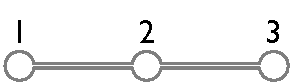
\includegraphics[width=.2\textwidth]{img/sample-1.pdf}

If you start in hall~$2$ and visit the rest of the halls in the order $2$, $1$, $2$, $3$, then you can switch off their machines at time~$0$ (in hall $2$), time~$1$ (in hall $1$), and time~$3$ (in hall $3$).
This wastes $0+1+3=4$~liters of liquid in total.
If instead you start in hall~$1$ and visit the halls in the order $1$, $2$, $3$, the total amount of liquid wasted is $0+1+2=3$~liters, which is better.

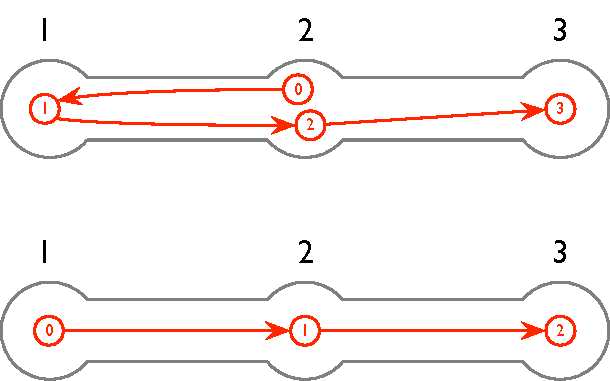
\includegraphics[width=.4\textwidth]{img/sample-1-ans.pdf}

\subsection*{Input}

The first line of input consists of the integer $n$, denoting the number of halls.
We assume that the halls are numbered $1$, $\ldots$, $n$.
The next $n-1$ lines each contain two space-separated integers $u$ and $v$ with 
$1\leq u < v \leq n$, % constraint:hallnames
meaning that there is a tunnel between hall~$u$ and hall~$v$.

\subsection*{Output}

Print a single integer: the minimum amount of spilled liquid, in liters.

\subsection*{Constraints and Scoring}

We always have
$1\leq n\leq 100\,000$. % constraint:n

Your solution will be tested on a set of test groups, each worth a number of points.
Each test group contains a set of test cases.
To get the points for a test group you need to solve all test cases in the test group.
Your final score will be the maximum score of a single submission.

\medskip
\begin{tabular}{lll}
Group & Points & Constraints \\\hline
1 & 18 & no hall is incident on more than two tunnels\\
2 & 19 & at most one hall is incident on more than two tunnels\\
3 & 20 & $n\leq 10$\\
4 & 21 & $n\leq 1000$\\
5 & 22 & \emph{no additional constraints}
\end{tabular}
